% !TEX TS-program = xelatex
% !TEX encoding = UTF-8

% This is a simple template for a XeLaTeX document using the "article" class,
% with the fontspec package to easily select fonts.
% test-xelatex.tex
%
% cleantex command is my friend! (a zsh script)
%

\documentclass[12pt]{article} % use larger type; default would be 10pt

\usepackage{fontspec} % Font selection for XeLaTeX; see fontspec.pdf for documentation
\defaultfontfeatures{Mapping=tex-text} % to support TeX conventions like ``---''
\usepackage{xunicode} % Unicode support for LaTeX character names (accents, European chars, etc)
\usepackage{xltxtra} % Extra customizations for XeLaTeX

\setmainfont{Charis SIL} % set the main body font (\textrm), assumes Charis SIL is installed
\setsansfont{DejaVuSans}
\setmonofont{DejaVuSansMono}

% other LaTeX packages.....
\usepackage{geometry} % See geometry.pdf to learn the layout options. There are lots.
\geometry{letterpaper} % or letterpaper (US) or a5paper or....
\geometry{margin=1.0in}
\usepackage[parfill]{parskip} % Activate to begin paragraphs with an empty line rather than an indent

\usepackage{graphicx} % support the \includegraphics command and options

\title{Testing a XeLaTeX Document}
\author{John Minter}
\date{\today} % Activate to display a given date or no date (if empty),
                       % otherwise the current date is printed 

\begin{document}
\maketitle

\begin{abstract}
This is a simple paragraph at the beginning of the document. A brief introduction to the main subject.
Let's try a mod to test .gitignore.
\end{abstract}

\section{Introduction}

\section{Section One}

\subsection{Sub One}

This line will start a second paragraph. And I can
 break\\ the lines \\ and continue on a new line.
 
The well known Pythagorean theorem \(x^2 + y^2 = z^2\) was 
proved to be invalid for other exponents. 
Meaning the next equation has no integer solutions:

\[ x^n + y^n = z^n \]

In physics, the mass-energy equivalence is stated 
by the equation $E=mc^2$, discovered in 1905 by Albert Einstein.

The mass-energy equivalence is described by the famous equation

\[E=mc^2\]

discovered in 1905 by Albert Einstein. 
In natural units ($c$ = 1), the formula expresses the identity

\begin{equation}
E=m
\end{equation}

\subsection{Sub Two}

Add a sub-section. Let's write a line that is long enough to wrap. I admit I get tired of writing 
these test cases. This means more editing to do a real document.  At some point I need to work
in a bibliography \ldots

\section{Section Two}

Let's insert a line of text here. It would wrap if long enough \ldots

\subsection{Sub One}

Let's try an image

The following image does not show any wombats, but does show cookies!



\begin{figure}[h!]
\begin{center}
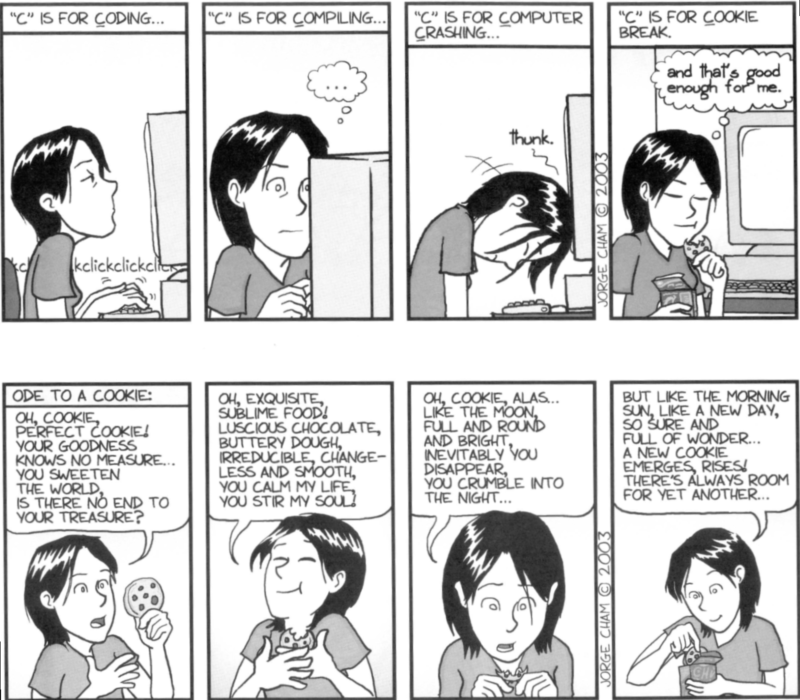
\includegraphics[width=0.7\textwidth]{./images/cookie.png}.
\caption{A picture of Cecelia from Ph. D. Comics. She is enjoying a tasty cookie!}
\end{center}
\end{figure}



%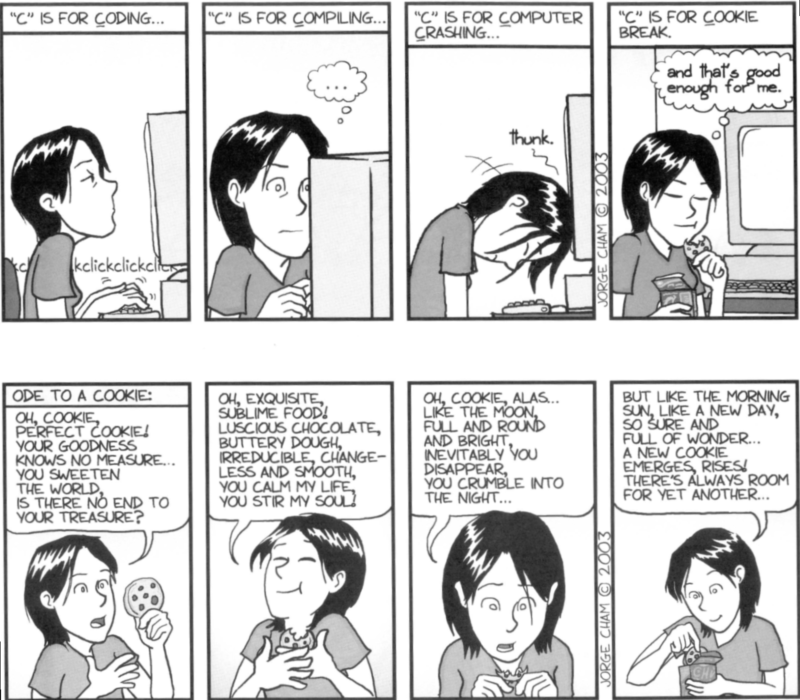
\includegraphics[height=\baselineskip]{./images/cookie.png}.

\subsection{Sub Two}


\end{document}